%Este trabalho está licenciado sob a Licença Creative Commons Atribuição-CompartilhaIgual 3.0 Não Adaptada. Para ver uma cópia desta licença, visite http://creativecommons.org/licenses/by-sa/3.0/ ou envie uma carta para Creative Commons, PO Box 1866, Mountain View, CA 94042, USA.

%%%%%%%%%%%%%%%%%%%%%%%%%%%%%%%%%
%   Predefinicoes
%%%%%%%%%%%%%%%%%%%%%%%%%%%%%%%%%
\newif\ifisslide       % O layout será slide (ou a4)?
\newif\ifisscilab      % As notas incluirão Scilab? 
\newif\ifisoctave      % As notas incluirão octave?

%\isslidetrue           % formato slide
\isslidefalse           % formato a4paper

\isscilabtrue           % incluir scilab
%\isscilabfalse         % não incluir

%\isoctavetrue          % incluir octave
\isoctavefalse          % não incluir


%%%%%%%%%%%%%%%%%%%%%%%%%%%%%%%%%
%   Opcões de Linguagem
%%%%%%%%%%%%%%%%%%%%%%%%%%%%%%%%%
\usepackage[brazil]{babel}
\usepackage[utf8]{inputenc}
\usepackage[T1]{fontenc}
%\usepackage{xunicode} é o pacote necessário para a codificação UTF-8 no XeTeX


%%%%%%%%%%%%%%%%%%%%%%%%%%%%%%%%%
%   Layout das páginas
%%%%%%%%%%%%%%%%%%%%%%%%%%%%%%%%%
\ifisslide
  \setlength{\paperwidth}{5in}%
  \setlength{\paperheight}{4in}%
  \usepackage[body={4.75in,3.65in},hmarginratio=1:1]{geometry}[2002/07/08]
\else
  \usepackage[a4paper,headheight=15.4pt]{geometry}
  %\usepackage[hmargin=2.5cm,vmargin=2.5cm]{geometry}
\fi

\usepackage{fancyhdr}
% \pagestyle{fancyplain}
% \lhead[\fancyplain{}{\thepage}]%
%   {\fancyplain{}{\em\rightmark}}
% \rhead[Cálculo Numérico]%
%   {\fancyplain{}{\thepage}}
\pagestyle{fancy}
\fancyhf{}
\fancyhead[RE]{Cálculo Numérico}
\fancyhead[LO]{\rightmark}
\fancyhead[LE,RO]{\thepage}

%license footnote
\cfoot{\tiny{Licença CC-BY-SA-3.0. Contato: \url{livro_colaborativo@googlegroups.com}}}

%%%% no blank pages between chapters %%%%
\let\cleardoublepage\clearpage



%%%% independent chapters %%%%
\usepackage{subfiles}


%%%% ams-latex %%%%
\usepackage{amsmath}
\usepackage{amssymb}
\usepackage{amsthm}

%%%% graphics %%%%
\usepackage{graphics}
\usepackage{graphicx}
\usepackage{caption}
\usepackage{subcaption}

%%%% links %%%%
\usepackage[hidelinks]{hyperref}

%%%% copy and paste from PDF (correctly) %%%%
\usepackage{upquote}
\usepackage{lmodern}

%%%% code insert (verbatim) %%%%
\usepackage{verbatim}

%%%% indent first line %%%%
\usepackage{indentfirst}

%%%% comma as a decimal separator %%%%
\usepackage{icomma}

%%%% citation %%%%
\usepackage{cite}

%%%% miscellaneous %%%%
\usepackage{multicol}
\usepackage{multirow}
\usepackage[normalem]{ulem}
\renewcommand{\arraystretch}{1.5} %space between rows in tables

%%%%%%%%%%%%%%%%%%%%%%%%%%%%%%%
%%%% Exercises and Answers %%%%
\usepackage[answerdelayed,lastexercise]{exercise}
\usepackage{chngcntr}
\counterwithin{Exercise}{section}
\counterwithin{Answer}{section}
\renewcommand{\ExerciseHeaderTitle}{({\it \ExerciseTitle})}
\renewcommand{\ExerciseName}{E}
\renewcommand{\ExerciseHeader}{{\textbf{\large\ExerciseName~\ExerciseHeaderNB\ExerciseHeaderTitle\ExerciseHeaderOrigin}}}
\renewcommand{\ExerciseHeader}{\textbf{\ExerciseName\ \ExerciseHeaderNB.}\,}

% change font for answers header
\renewcommand{\AnswerHeader}{\tiny\textbf{\ExerciseName\ \ExerciseHeaderNB.}\smallskip}
% change font for answers list header
\renewcommand{\AnswerListHeader}{{\tiny\textbf{\AnswerListName\
(\ExerciseListName\ \ExerciseHeaderNB)\ ---\ }}}
%%%%%%%%%%%%%%%%%%%%%%%%%%%%%%


%%%%%%%%%%%%%%%%%%%%%%%%%%%%%%%%%
%   Formatacoes de estilo
%%%%%%%%%%%%%%%%%%%%%%%%%%%%%%%%%
\usepackage{xcolor}
\newcommand{\RED}[1]{{\color{red}{#1}}}
\newcommand{\BLU}[1]{{\color{blue}{#1}}}
\newcommand{\GRE}[1]{{\color{darkgreen}{#1}}}

%emphasis \emph
\DeclareTextFontCommand{\emph}{\bfseries}

\newcommand{\sen}{\operatorname{sen}\,}
\newcommand{\tg}{\operatorname{tg}\,}
\newcommand{\p}{\partial}
\newcommand{\Dom}{\operatorname{Dom}\,}


%%%%%%%%%%%%%%%%%%%%%%%%%%%%%%%%%
%  ambientes 
%%%%%%%%%%%%%%%%%%%%%%%%%%%%%%%%%
\ifisslide
  \input preambulo_slide.tex
\else
  \theoremstyle{plain}          %   bold title, italic body
  \newtheorem{teo}{Teorema}[section]
  \newtheorem{lem}{Lema}[section]
  \newtheorem{prop}{Proposição}[section]
  \newtheorem{corol}{Corolário}[section]
  \newtheorem{defn}{Definição}[section]
  \theoremstyle{remark}           % italic title, romman body
  \theoremstyle{definition}       % italic title, romman body
  \newtheorem{obs}{Observação}[section]
  \newtheorem{ex}{Exemplo}[section]
\fi

\newenvironment{sol}
{\let\oldqedsymbol=\qedsymbol
  \renewcommand{\qedsymbol}{$\Diamond$}
  \begin{proof}[\bfseries\upshape Solução]}
  {\end{proof}
  \renewcommand{\qedsymbol}{\oldqedsymbol}}



%%%% indexing %%%%
\usepackage{makeidx}
\makeindex



%%%% titlepage figure %%%%
\usepackage{eso-pic}
\newcommand\BackgroundPic{%
\put(0,0){%
\parbox[b][\paperheight]{\paperwidth}{%
\vfill
\centering
\includegraphics[width=\paperwidth,height=\paperheight,%
keepaspectratio]{./rosto/capa.eps}%
\vfill
}}}

%%%%% macros  %%%%%%%%%%%%%
\newcommand{\matdd}[4]{\begin{bmatrix} #1&#2\\#3&#4 \end{bmatrix}}
\newcommand{\matddd}[9]{\begin{bmatrix} #1&#2&#3 \\ #4&#5&#6 \\ #7&#8&#9 \end{bmatrix}}
\newcommand{\vetdd}[2]{\begin{bmatrix} #1 \\#2 \end{bmatrix}}
\newcommand{\vetddd}[3]{\begin{bmatrix} #1 \\ #2\\ #3 \end{bmatrix}}
